%%%%%%%%%%%%%%%%%%%%%%%%%%%%%%%%%%%%%%%%%%%%%%%%%%%%%%%%%%%%%%%%%%%%%%%%%%%%%%%
%     enunciado.tex:    Enunciado de la pr�ctica 2 de GIEAI-Inform�tica
%%%%%%%%%%%%%%%%%%%%%%%%%%%%%%%%%%%%%%%%%%%%%%%%%%%%%%%%%%%%%%%%%%%%%%%%%%%%%%%

\documentclass[english,a4paper,11pt]{article}

\usepackage[latin1]{inputenc}  % codificaci�n de caracteres de este archivo
\usepackage[spanish]{babel}    % Traducir: ``abstract'' ---> ``resumen''   etc.
\usepackage{fancyhdr}          % p�ginas con cabecera y pie
\usepackage{listings}          % listados de c�digo fuente
\usepackage{float}             % para que los listados floten como las figuras
\usepackage{vmargin}           % ajuste de m�rgenes f�cil de usar
\usepackage[T1]{fontenc}       % meter fuentes vectoriales
\usepackage{graphicx}          % figuras
\usepackage{upquote}           % comilla recta con \textquotesingle
\usepackage{placeins}          % orden \FloatBarrier para mantener figuras a raya

\usepackage[implicit=false]{hyperref}  % enlaces web (el par�metro implicit=false
                                       % evita problemas con el # de #include etc.)
                                       % uso expl�cito: \href[options]{URL}{text}
                                       %                \url{URL}

% mis abreviaturas
\newcommand{\C}{\texttt{C}}            % escribir� \C en lugar de \texttt{C}
\newcommand{\Pascal}{\texttt{Pascal}}  % idem con \Pascal ...
\newcommand{\fun}[1]{\texttt{#1()}}    % "\fun{main}" ---> "main()" en letra typewriter
\newcommand{\hex}[1]{\texttt{#1}$_{hex}$}
\newcommand{\bin}[1]{\texttt{#1}$_{bin}$}
\newcommand{\enesimo}{\mbox{n-�simo}}
\newcommand{\muvision}{\textit{$\mu\!$Vision4}}
\newcommand{\keilmuvision}{\textit{Keil}~\muvision}
\newcommand{\codigo}[1]{\texttt{#1}}
\newcommand{\menu}[1]{\textit{#1}}

% �rdenes para alternar entre el estilo espa�ol (ligera separaci�n extra
% entre p�rrafos) y el estilo por defecto (p�rrafos junticos junticos)
\newcommand{\parrafosjuntos}{\setlength{\parskip}{0pt}}
\newcommand{\parrafosseparados}{\setlength{\parskip}{1.5ex plus 0.6ex minus 0.5ex}}

% datos importantes del documento
\newcommand{\titulo}{Understanding parameters settings in Evolutionary Algorithms}     % <<--- T�TULO
\newcommand{\fecha}{}                         % <<--- TEMA
\newcommand{\asignatura}{IASCA}
\newcommand{\institucion}{Departamento de Autom�tica, UAH}
\newcommand{\paginaweb}{http://atc1.aut.uah.es}

% portada
\title{\asignatura \\ \titulo}
\author{\institucion \\ \url{\paginaweb}}
\date{\fecha}

% m�rgenes un poco m�s finos
\setmargrb{25mm}{20mm}{25mm}{20mm}    % left, top, right, bottom

% encabezado y pie
\pagestyle{fancy}
\lhead{\footnotesize \parbox{11cm}{\asignatura}}
\lfoot{\footnotesize \parbox{11cm}{\institucion}}
\cfoot{}
\rhead{\footnotesize \titulo}
\rfoot{\footnotesize P�gina \thepage}
\renewcommand{\headheight}{24pt}
\renewcommand{\footrulewidth}{0.4pt}
%\renewcommand{\headrulewidth}{0pt}

% listados de c�digo fuente flotantes
%\newfloat{floatlisting}{h}{}
%\floatname{floatlisting}{Listado}

% estilo de los listados de c�digo
\lstset{numbers=left,                 % n�meros de l�nea
        numberstyle=\tiny,            % tama�o de los num. de l�nea
        extendedchars=true,           % acentos, e�es...
        %frame=single,                 % marco que encuadra al listado
        basicstyle=\footnotesize\ttfamily,   % tipo de letra
        showstringspaces=false}       % no mostrar espacios de las cadenas

\graphicspath{{figs/}}                % ruta de las figuras

\begin{document} % ------------------ Aqu� empieza el documento ----------------------

% redefinir el nombre de algunas cosas
\renewcommand{\tablename}{Tabla}                  % mejor "Tabla" que "Cuadro"
\renewcommand{\listtablename}{Indice de tablas}
% definidos originalmene en:
%/usr/share/texmf-texlive/tex/generic/babel/spanish.ldf

\maketitle              % montar el t�tulo aqu�� con los par�metros definidos arriba
\thispagestyle{empty}   % no poner n�mero de p�gina ni nada de nada en la 1� p�gina

\renewcommand{\abstractname}{}         % eliminar "Resumen"
\begin{abstract}                       % resumen (sin la palabra "Resumen")
\noindent \textbf{Objectives:}
\begin{itemize}
\item Introduce \texttt{inspyred}
\item Understand the parameter settings of a basic GA
\item Observe the basic behaviour of an EA
\item Customize the parameter settings
\item Gather and process the main statistics
\end{itemize}
\end{abstract}

\sloppy              % hacer m�s flexible el c�lculo del espacio entre palabras para
                     % evitar errores de tipo "overfull box"
                     % (lo contrario de \sloppy es \fussy)

\parrafosseparados   % separaci�n entre p�rrafos (por defecto saldr�n pegados)

\subsection*{Preliminary steps}
Install \textit{inspyred} following the instructions available on \url{http://pythonhosted.org/inspyred/}. Basically, \textit{inspyred} is a Python module that can be installed like any other module. From an Unix console, just type \textit{pip install inspyred}.

\subsection*{One-max problem with Genetic Algorithm}

Copy or download the following script, which implements the one-max problem with a basic Genetic Algorithm. All the relevant algorithm parameters are contained in variables defined in the begining of the script.

\lstinputlisting{code/onemax.py}

The parameter setting used is the following one:

\begin{itemize}
	\item Representation: Binary
	\item Chromosome length: 15
	\item Crossover: 1-point crossover
	\item Mutation: Flip mutation
	\item Mutation probability: 0.1
	\item Population size: 50
	\item Termination: 15 generations
\end{itemize}

Perform the following tasks:

\begin{enumerate}
	\item Execute the script to validate the installation of \textit{inspyred}.
	\item Observe how average and best fitness evolve along the time. Explain their behavior.
	\item Execute the script several times, did it always find the solution? Why?
	\item Change the chromosome length to $30$ and repeat the previous questions.
	\item Customize the algorithm settings to increase the probability of finding a solution.
	\item Set $p_m=0.5$. What happen?
	\item Set $p_m=1.0$. What happen?
	\item Set the chromosome length to $50$ and customize the algorithm to increase the probability of finding a solution.
\end{enumerate}

\subsection*{Optimization problem}

Sound comparison of EAs is a thought problem. In order to make this task easier there is a number of theoretical problems\footnote{You will find several names in the literature, such as benchmark problems or DeJong's functions, however the latter is a fixed collection of $12$ functions.} that are commonly used to assess the performance of new algorithms. These problems have different properties and, together, offer a base to make comparisons. The next figure shows some of the most common benchmark problems used in EC.

\begin{center}
\centering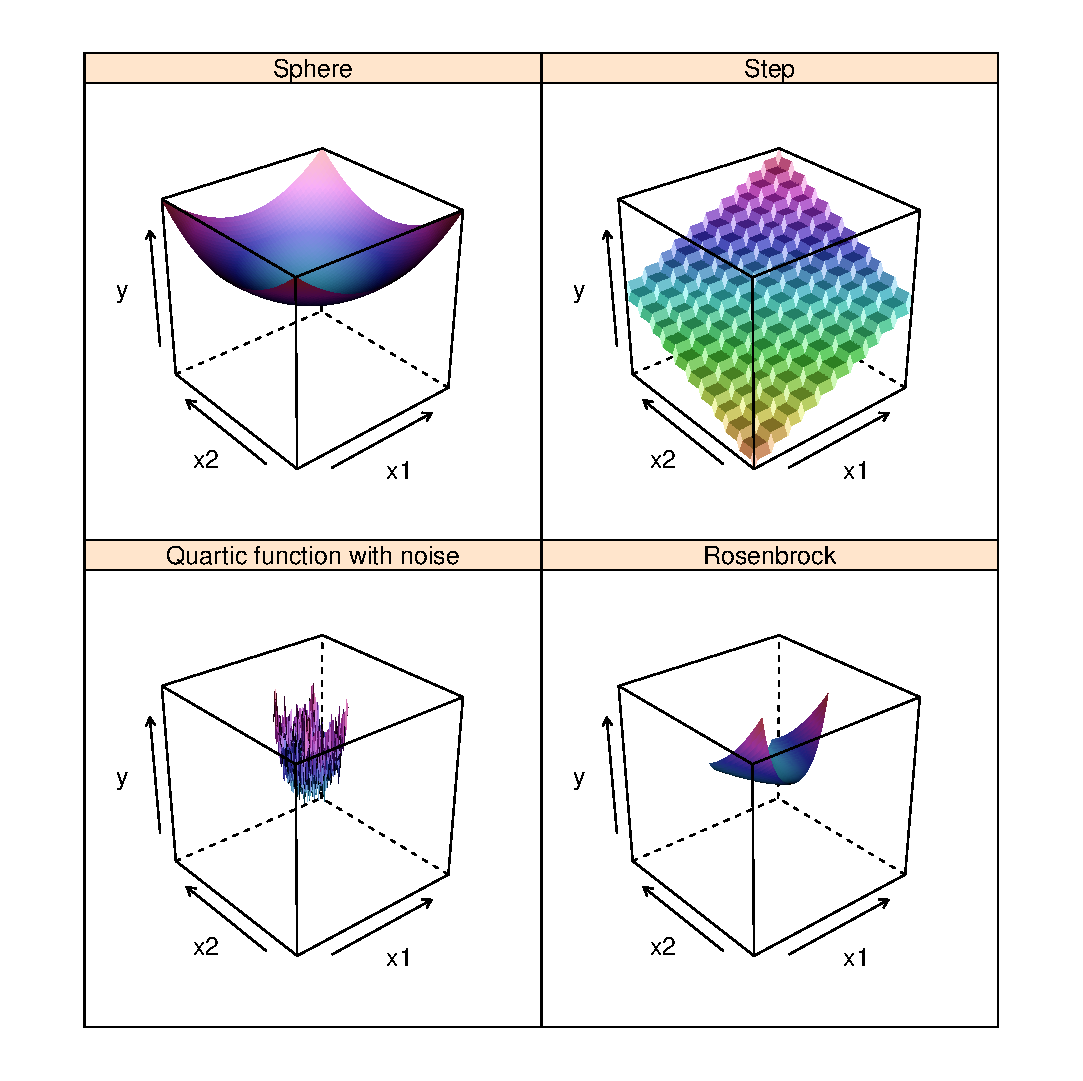
\includegraphics[width=0.6\linewidth]{figs/deJong.eps}
\end{center}

In this exercise we will use one of these, the Schwefel problem, that can be formally stated as follows:

\begin{equation}
f(x) = 418.9829n - \sum_{i=1}^n \left[-x_i \sin(\sqrt{|x_i|})\right]
\end{equation}

where $n$ represents the number of dimensions and $x_i \in [-500, 500] \forall i=1,...,n$. The input values that optimizes the function is $[420.9687, 420.9687, ..., 420.9687]$, this a minimaization task and the best fitness is $0$. A graphical representation of this problem for $n=2$ (two dimensions) follows.

\begin{center}
\centering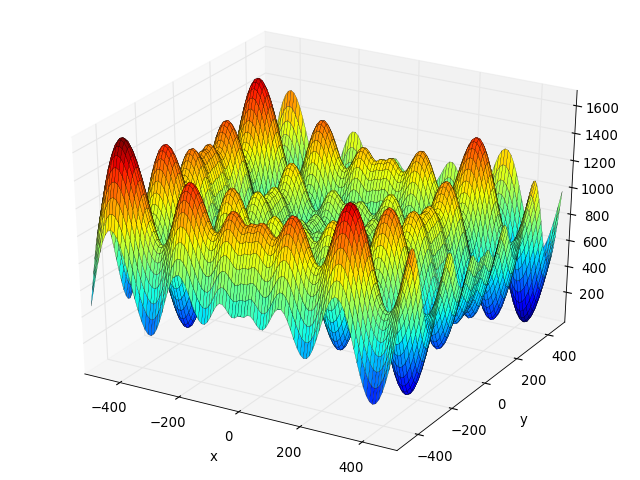
\includegraphics[width=0.6\linewidth]{figs/schwefel.png}
\end{center}

The code that implemens a GA that solves the Schwefel problem is the next listing. Observe that the main algorithm parameters have been deleted.

\lstinputlisting{code/ga_example.py}

The algorithm design is as follows.

\begin{itemize}
	\item Representation: Binary
	\item Chromosome length: 30
	\item Crossover: n-point crossover
	\item Mutation: Flip mutation
	\item Mutation probability: X
	\item Population size: X
	\item Termination: 8,000 evaluations
\end{itemize}


Copy or download the code and perform the following task:

\begin{enumerate}
	\item Set the parameters to get a perfect solution (fitness=$0$).
	\item Set the parameters to get the solution as soon as possible.
	\item Execute the algorithm $10$ times and show a graph relating generation, best fitness and average fitness. To obtain the graph values, average across all the $10$ runs. If necessary, change the code and use any external tool (Excel, Matlab, R, Gnuplot, ...) at your convenience.
\end{enumerate}

\subsection*{Symbolic regression with Genetic Programming (non-inspyred exercise)}
Regression is a classical problem in Machine Learning. If you understand the classical lineal regression, you already know what the regression problem is. Given a set of samples drawn from a function, the problem is to find the symbolic representation of that function. The range of applications is huge, financial modelling or whaether forecasting, may serve as examples. A function has a non-linear nature, and is well represented by trees, so, not surprisingly GP is widely use to tackle this kind of problems.

In regression the fitness uses to be the  mean squared error (MSE), which is defined as $MSE=\frac{1}{n}\sum{i=1}^{n}(\bar{Y}_i - Y_i)$ where $\bar{Y}_i$ is the observed value and $Y_i$ the theoretical one. So, regression is a minimization problem.

Unfortunately, \textit{inspyred} does not support GP, so we are going to use an on-line application. Open the site \url{http://alphard.ethz.ch/gerber/approx/default.html} with a Java enabled browser (i.e. do not use Chrome). If you have problems to execute the applet, open Java settings in your OS and give execution permissions to the applet.

\begin{center}
\begin{figure}
\centering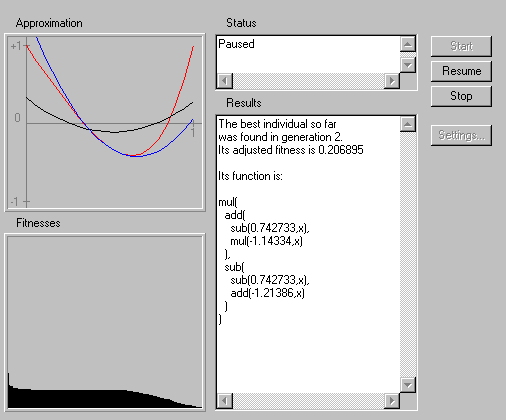
\includegraphics[width=0.6\linewidth]{figs/applet.png}
\caption{Applet with GP solving a symbolic regression problem.}
\end{figure}
\end{center}

The applet shows the target function (red), the best solution in run (blue) and the tree being assessed (black). It also represents the fitness histogram and a dump of the best tree found in the run. The most common GP parameters can be set with the button (Settings...).

Perform the follwing task:

\begin{itemize}
	\item Work in groups of two or three people. Compete with your colleagues to get the best approximation (i.e. the lowest fitness). Try with different parameters, including terminal and function sets.
\end{itemize}


\end{document}
